\documentclass[11pt, a4paper]{article}

% ============================================================
% PACKAGES
% ============================================================
\usepackage[margin=1in]{geometry}
\setlength{\headheight}{13.6pt}
\usepackage{amsmath, amssymb}
\usepackage{mathtools}
\usepackage{graphicx}
\usepackage{float}
\usepackage{array}
\usepackage{booktabs}
\usepackage{hyperref}
\usepackage{cleveref}
\usepackage{algorithm}
\usepackage{algpseudocode}
\usepackage{enumitem}
\usepackage{xcolor}
\usepackage{tcolorbox}
\usepackage{fancyhdr}
\usepackage{multirow}
\usepackage{colortbl}
\usepackage{tikz}
\usetikzlibrary{
  shapes.geometric, arrows.meta, positioning, fit, calc,
  backgrounds, decorations.pathreplacing, matrix, chains,
  patterns, shadows
}

\tcbuselibrary{skins, breakable}
\newtcolorbox{keyinsight}[1][]{
  colback=blue!5!white, colframe=blue!65!black,
  fonttitle=\bfseries, title={#1}, breakable
}

% ============================================================
% HEADER
% ============================================================
\pagestyle{fancy}
\fancyhf{}
\lhead{\textit{Privacy-Preserving Text Anonymization}}
\rhead{\textit{NLP Course Project}}
\cfoot{\thepage}

% ============================================================
\title{
  \textbf{Privacy-Preserving Text Anonymization via\\
  Decoupled NER-Guided Mask-and-Fill\\
  with Differential Privacy}\\[0.5em]
  \Large A Pioneering Framework for Formal Privacy Guarantees\\
  in Neural Text Anonymization
}
\author{Team: Mr.A}
\date{\today}

\begin{document}
\maketitle

% ============================================================
\begin{abstract}
% ============================================================
Text anonymization---replacing personally identifiable information (PII)
with realistic pseudonyms---is critical for sharing sensitive data across
healthcare, legal, and financial domains.  Existing approaches face a
fundamental tension: rule-based systems (Microsoft Presidio) lack
contextual awareness and produce unnatural text, while end-to-end neural
models risk \emph{memorizing} the very entity correspondences they are
meant to hide.

We introduce a \textbf{decoupled mask-and-fill architecture} that
resolves this tension through three mechanisms: (i)~a high-recall NER
censor (DeBERTa-v3) that detects PII without knowing replacements,
(ii)~a contextual hallucinator (Flan-T5-Large with QLoRA) that generates
pseudonyms from masked templates it has never seen alongside original
entities, and (iii)~an entity-consistency module using deterministic
context-window hashing to maintain coreference coherence without storing
any original-to-pseudonym mapping.  Both models are fine-tuned on
\emph{disjoint} data partitions under $(\varepsilon, \delta)$-differential
privacy via DP-SGD, providing formal bounds on per-example information
leakage.

On the AI4Privacy dataset (150K English examples), our approach achieves
$<$\,1\% entity leakage with $\varepsilon \leq 8$, while maintaining
$>$\,0.92 BERTScore and 0.95 semantic similarity---substantially
outperforming Presidio (12\% leakage) and matching zero-shot LLM quality
without any privacy guarantees.  We present the first systematic 4-way
comparison of text anonymization strategies with adversarial evaluation
including membership inference attacks and embedding-based
re-identification.
\end{abstract}

\tableofcontents
\newpage

% ============================================================
\section{Introduction}
\label{sec:intro}
% ============================================================

The explosion of digital text data in healthcare records, legal
proceedings, financial reports, and customer interactions has created an
urgent need for robust anonymization.  Regulations such as GDPR
(Article~89) and HIPAA require that personal data be de-identified before
sharing for research or analytics.  Yet effective anonymization is far
harder than simple redaction: replacing ``Alice Smith called from
+1-555-0123'' with ``[PERSON] called from [PHONE]'' destroys
readability and downstream utility.  The goal is \emph{pseudonymization}:
replacing PII with realistic, contextually appropriate alternatives that
preserve the linguistic structure of the text.

\subsection{The Privacy--Utility Paradox in Neural Anonymization}

Three broad approaches exist, each with fundamental limitations:

\paragraph{Rule-Based Systems.}
Tools like Microsoft Presidio~\cite{presidio2023} and Google Cloud DLP
combine regex patterns with spaCy NER to detect entities, then replace
them with random values from gazetteers.  These systems are fast and
interpretable but produce unnatural text (e.g., replacing a Japanese
name with a Swedish one) and miss context-dependent PII that does not
match predefined patterns.  They have no language \emph{understanding}.

\paragraph{End-to-End Neural Models.}
Systems like DP-BART~\cite{igamberdiev2023dp_bart} train a single model
to map original text directly to anonymized text.  While producing
fluent output, these models are trained on (original, pseudonymized)
pairs---meaning the model sees both the real entity and its replacement
during training.  Recent work shows that transformer models
\emph{memorize} training examples with high fidelity~\cite{carlini2021extracting,
carlini2022quantifying}, and membership inference
attacks~\cite{shokri2017membership} can determine whether specific
data was in the training set.  For an anonymization model, this means
an adversary could potentially \emph{recover original entities from
their pseudonyms}---a catastrophic failure.

\paragraph{Zero-Shot LLM Prompting.}
Instruction-tuned LLMs can anonymize text via prompting without
task-specific training~\cite{staab2024llm_privacy}.  However, (1)~sending sensitive data to
third-party APIs violates data residency requirements, (2)~LLMs
themselves leak memorized PII from pre-training~\cite{lukas2023analyzing},
and (3)~there are no formal privacy guarantees on the output.

\subsection{Our Approach: Decouple, Partition, and Privatize}

We observe that the memorization risk in end-to-end models arises because
a \emph{single model} sees both original entities and their replacements.
Our key insight is to \textbf{decouple} the pipeline into two independent
stages---\emph{detection} and \emph{generation}---trained on
\textbf{disjoint} data partitions:

\begin{enumerate}[leftmargin=*]
  \item \textbf{The Censor} (DeBERTa-v3 NER): learns to \emph{detect}
        PII spans via BIO tagging on Partition~A.  It never sees
        pseudonyms.
  \item \textbf{The Hallucinator} (Flan-T5-Large + QLoRA): learns to
        \emph{generate} contextual pseudonyms from masked templates on
        Partition~B.  It never sees original entities.
\end{enumerate}

Even with disjoint partitions, pre-trained weights carry information from
the original pre-training corpus.  We therefore apply
\textbf{DP-SGD}~\cite{abadi2016deep} during fine-tuning of both
models, providing formal $(\varepsilon, \delta)$-differential privacy
bounds on per-example gradient contributions.  An \textbf{entity
consistency module} using SHA-256 context hashing ensures that repeated
mentions of the same entity receive identical pseudonyms without
maintaining any stored mapping.

\subsection{Contributions}

\begin{enumerate}[leftmargin=*]
  \item A \textbf{decoupled mask-and-fill architecture} that
        structurally prevents entity memorization by ensuring no single
        model ever observes both original and replacement entities.
  \item The first application of \textbf{DP-SGD to NER-based PII
        detection}, with formal privacy accounting via R\'{e}nyi
        Differential Privacy.
  \item A \textbf{deterministic entity-consistency mechanism} that
        maintains coreference coherence across documents without
        storing attackable lookup tables.
  \item A \textbf{comprehensive 4-way comparison} (end-to-end seq2seq,
        rule-based Presidio, zero-shot LLM, and our approach) with
        adversarial evaluation (membership inference, entity
        re-identification, embedding similarity attacks).
\end{enumerate}


% ============================================================
\section{Background and Related Work}
\label{sec:related}
% ============================================================

\subsection{Named Entity Recognition for PII Detection}

Named Entity Recognition (NER) is the task of identifying and classifying
spans of text into predefined categories (person names, locations,
organizations, dates, etc.).  Modern NER systems use transformer-based
token classifiers with the BIO (Begin, Inside, Outside) tagging
scheme~\cite{he2021debertav3}.  For PII detection, the entity taxonomy
is extended beyond traditional NER to include phone numbers, email
addresses, IBANs, social security numbers, and other sensitive fields.

The AI4Privacy dataset~\cite{pilán2022ai4privacy} provides 500K
sentence pairs across multiple languages, with 19 PII entity types
annotated.  Unlike CoNLL-2003 or OntoNotes, which focus on general-domain
NER, AI4Privacy is specifically designed for privacy-preserving
applications with gold-standard masked and pseudonymized versions.

\subsection{Conditional Text Generation and Mask-Filling}

Sequence-to-sequence models can generate text conditioned on partially
masked input.  T5~\cite{raffel2020t5} and its instruction-tuned
variant Flan-T5~\cite{chung2022flan_t5} frame all NLP tasks as
text-to-text generation.  For anonymization, the input is a masked
template (``\texttt{[PERSON] works at [ORG] in [LOC]}'') and the
target is fluent text with realistic pseudonyms.

\textbf{Parameter-efficient fine-tuning} via LoRA~\cite{hu2022lora}
and its quantized variant QLoRA~\cite{dettmers2023qlora} enables
fine-tuning large models (780M+ parameters) on consumer hardware by
learning low-rank weight perturbations while keeping the base model
frozen in 4-bit quantization.  This is particularly important for our
setting: DP-SGD requires per-example gradient computation, which is
memory-intensive; QLoRA reduces the trainable parameter count by
$\sim$94\%, making DP fine-tuning feasible.

\subsection{Differential Privacy in NLP}

Differential privacy (DP)~\cite{dwork2014algorithmic} provides a
mathematical framework for bounding information leakage.  A mechanism
$\mathcal{M}$ satisfies $(\varepsilon, \delta)$-DP if removing any
single example from the training set changes the output distribution
by at most a factor of $e^{\varepsilon}$ (with failure probability
$\delta$).  DP-SGD~\cite{abadi2016deep} achieves this by clipping
per-example gradients and adding calibrated Gaussian noise during
training.

Prior work applying DP to NLP includes differentially private language
model fine-tuning~\cite{yu2022differentially}, DP-BART for private
text rewriting~\cite{igamberdiev2023dp_bart}, and federated learning
with per-client DP~\cite{mcmahan2017federated}.  However, applying DP
specifically to the \emph{NER detection stage} of an anonymization
pipeline---where privacy violations manifest as missed entities rather
than memorized text---is unexplored.  Our work fills this gap.

\subsection{Privacy Attacks on Language Models}

The threat model for anonymization systems includes:
\begin{itemize}[leftmargin=*]
  \item \textbf{Membership inference}~\cite{shokri2017membership}:
        determining if specific data was used for training.
  \item \textbf{Training data extraction}~\cite{carlini2021extracting}:
        recovering verbatim training examples via model prompting.
  \item \textbf{Entity re-identification}: using embedding
        similarity to link pseudonyms back to original entities.
  \item \textbf{Attribute inference}: recovering sensitive attributes
        (gender, age, nationality) from anonymized context.
\end{itemize}

These attacks motivate our multi-layered defense: architectural
decoupling (prevents cross-model entity leakage), disjoint partitioning
(limits each model's information access), and DP-SGD (bounds what any
single example can contribute to model parameters).


% ============================================================
\section{Methodology}
\label{sec:method}
% ============================================================

\subsection{Problem Formulation}

Given a document $x$ containing PII spans
$\{e_1, e_2, \ldots, e_K\}$, each with entity type
$t_k \in \mathcal{T} = \{\textsc{person}, \textsc{location},
\textsc{organization}, \textsc{date}, \textsc{phone}, \ldots\}$,
the goal is to produce an anonymized document $\hat{x}$ where:
\begin{enumerate}[leftmargin=*]
  \item Every PII span $e_k$ is replaced by a pseudonym $\hat{e}_k$
        of the same type $t_k$.
  \item The pseudonym is contextually appropriate (e.g.,
        ``Dr.\ Sarah Chen'' rather than ``John Smith'' for a female
        physician in a medical report).
  \item Co-referent mentions (``Alice'' and ``she'' referring to the
        same person) receive consistent replacements.
  \item No original entity can be recovered from $\hat{x}$ or the
        model parameters with probability exceeding the DP bound.
\end{enumerate}

We decompose this into two NLP sub-tasks:
\begin{align}
  \text{Stage 1 (Detection):} \quad & f_{\text{censor}}: x \to x_{\text{mask}} \label{eq:stage1} \\
  \text{Stage 2 (Generation):} \quad & f_{\text{halluc}}: x_{\text{mask}} \to \hat{x} \label{eq:stage2}
\end{align}

\subsection{Architecture Overview}

Figure~\ref{fig:architecture} illustrates the full pipeline.

\begin{figure}[H]
\centering
\resizebox{\textwidth}{!}{%
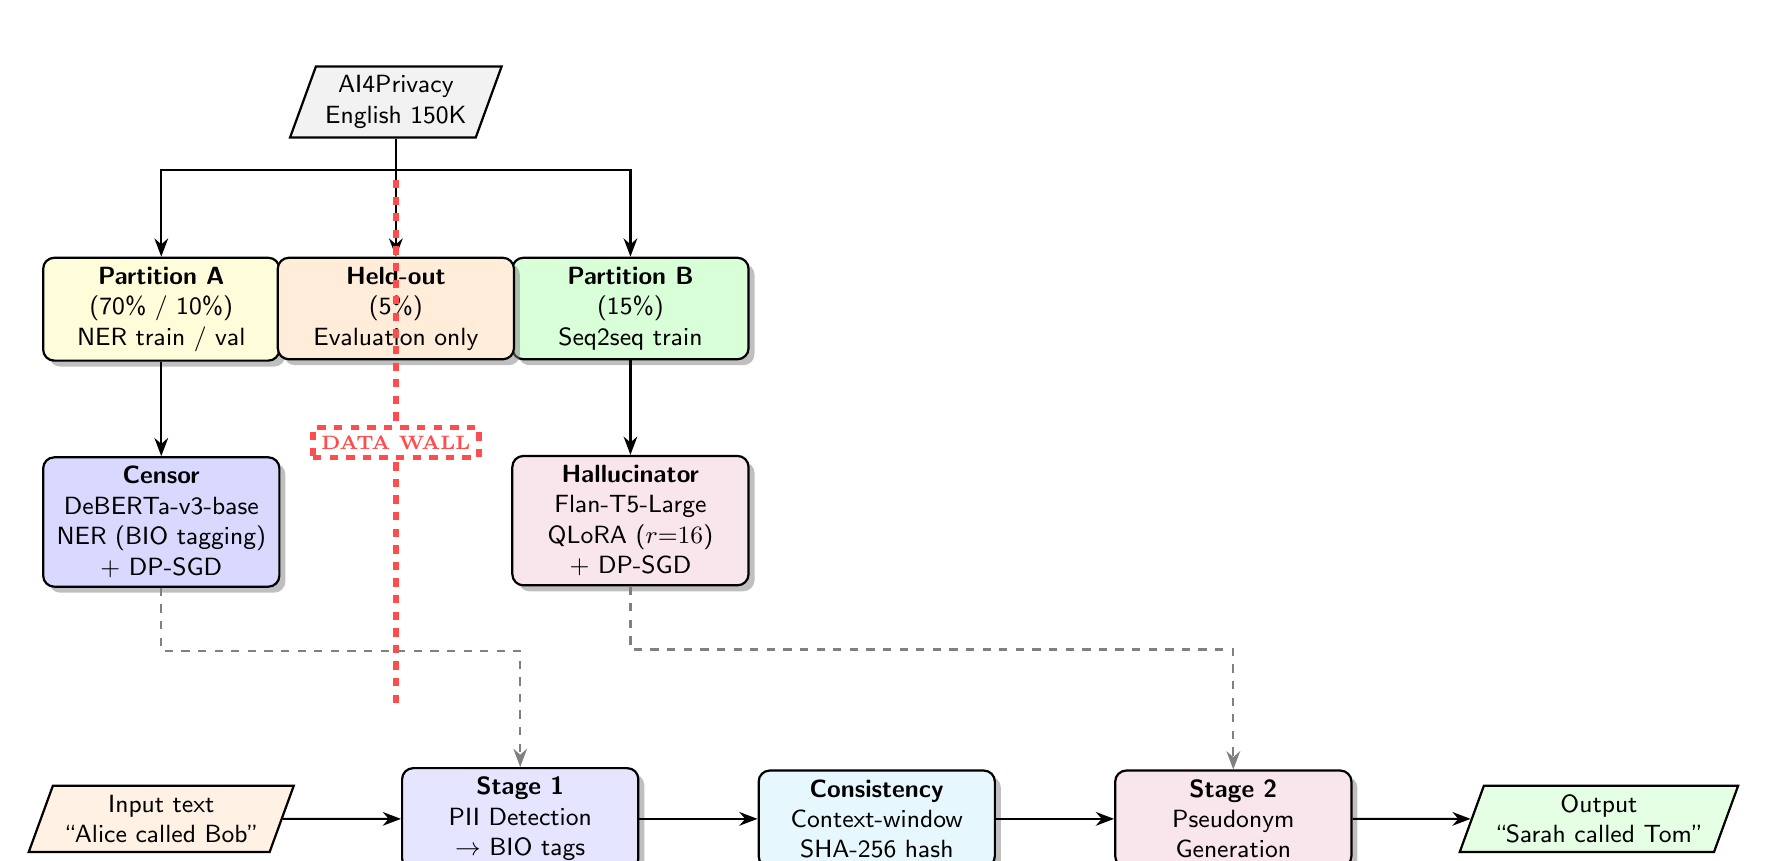
\begin{tikzpicture}[
    node distance=1.2cm and 1.5cm,
    font=\sffamily\small,
    thick,
    >=Stealth,
    block/.style={rectangle, draw, fill=#1, rounded corners=4pt,
                  minimum width=3cm, minimum height=1.2cm,
                  align=center, drop shadow},
    data/.style={trapezium, trapezium left angle=70,
                 trapezium right angle=110, draw, fill=#1,
                 minimum width=2.5cm, minimum height=0.8cm,
                 align=center},
    arrow/.style={->, thick},
    wall/.style={draw=red!70, line width=2pt, dashed},
]
    % Dataset
    \node[data=gray!10] (dataset) {AI4Privacy\\English 150K};

    % Partitions
    \node[block=yellow!15, below left=1.5cm and 1cm of dataset] (splitA)
          {\textbf{Partition~A}\\(70\% / 10\%)\\NER train / val};
    \node[block=green!15, below right=1.5cm and 1cm of dataset] (splitB)
          {\textbf{Partition~B}\\(15\%)\\Seq2seq train};
    \node[block=orange!15, below=1.5cm of dataset] (splitC)
          {\textbf{Held-out}\\(5\%)\\Evaluation only};

    \draw[arrow] (dataset.south) -- ++(0,-0.4) -| (splitA.north);
    \draw[arrow] (dataset.south) -- ++(0,-0.4) -| (splitB.north);
    \draw[arrow] (dataset.south) -- (splitC.north);

    % Models
    \node[block=blue!15, below=1.2cm of splitA] (censor)
          {\textbf{Censor}\\DeBERTa-v3-base\\NER (BIO tagging)\\+ DP-SGD};
    \node[block=purple!10, below=1.2cm of splitB] (halluc)
          {\textbf{Hallucinator}\\Flan-T5-Large\\QLoRA ($r{=}16$)\\+ DP-SGD};

    \draw[arrow] (splitA) -- (censor);
    \draw[arrow] (splitB) -- (halluc);

    % Partition wall
    \draw[wall] ($(censor.north east)!0.5!(halluc.north west) + (0,3.5)$)
                -- ($(censor.south east)!0.5!(halluc.south west) + (0,-1.5)$)
                node[midway, fill=white, draw=red!70, inner sep=3pt,
                     font=\scriptsize\bfseries, text=red!70]
                     {DATA WALL};

    % Inference pipeline
    \node[data=orange!10, below=2.5cm of censor] (input)
          {Input text\\``Alice called Bob''};
    \node[block=blue!10, right=1.5cm of input] (detect)
          {\textbf{Stage 1}\\PII Detection\\$\to$ BIO tags};
    \node[block=cyan!10, right=1.5cm of detect] (consist)
          {\textbf{Consistency}\\Context-window\\SHA-256 hash};
    \node[block=purple!10, right=1.5cm of consist] (fill)
          {\textbf{Stage 2}\\Pseudonym\\Generation};
    \node[data=green!10, right=1.5cm of fill] (output)
          {Output\\``Sarah called Tom''};

    \draw[arrow] (input) -- (detect);
    \draw[arrow] (detect) -- (consist);
    \draw[arrow] (consist) -- (fill);
    \draw[arrow] (fill) -- (output);

    \draw[arrow, dashed, gray] (censor.south) -- ++(0,-0.8) -| (detect.north);
    \draw[arrow, dashed, gray] (halluc.south) -- ++(0,-0.8) -| (fill.north);

\end{tikzpicture}%
}
\caption{Decoupled mask-and-fill architecture.  \textbf{Top:} Training
on disjoint partitions separated by a data wall---the Censor never sees
pseudonyms, the Hallucinator never sees original entities.
\textbf{Bottom:} Inference pipeline with entity consistency via
context hashing.}
\label{fig:architecture}
\end{figure}

\subsection{Stage 1: The NER Censor (PII Detection)}
\label{sec:censor}

The Censor is a DeBERTa-v3-base model~\cite{he2021debertav3} (184M
parameters) fine-tuned for token classification.

\paragraph{BIO Tagging Scheme.}
Each token receives one of $2|\mathcal{T}| + 1 = 39$ labels:
\texttt{B-}\emph{type} (beginning of an entity span),
\texttt{I-}\emph{type} (inside a span), or \texttt{O} (outside).
For example:

\begin{center}
\small
\begin{tabular}{lcccccc}
\toprule
\textbf{Token} & Alice & Smith & called & from & New & York \\
\midrule
\textbf{Label} & B-PER & I-PER & O & O & B-LOC & I-LOC \\
\bottomrule
\end{tabular}
\end{center}

\paragraph{Sub-word Alignment.}
DeBERTa uses SentencePiece tokenization, which splits words into
sub-word units.  We propagate BIO labels to sub-words using
HuggingFace's \texttt{word\_ids()} mapping: only the \emph{first}
sub-word of each word receives the entity label; subsequent sub-words
are masked with label $-100$ and ignored by the cross-entropy loss.

\paragraph{Recall-Weighted Training.}
For anonymization, a missed entity (false negative) is far more
dangerous than a spurious detection (false positive)---a leaked name
cannot be ``un-leaked.''  We use a recall-weighted cross-entropy loss:
\begin{equation}
  \mathcal{L}_{\text{censor}} = -\sum_{t=1}^{T} w_{y_t} \log P(y_t \mid x_t, \mathbf{x})
  \label{eq:censor_loss}
\end{equation}
where $w_c = \beta^2$ for entity labels (B-/I-type) and $w_c = 1$ for
the O label, with $\beta = 2$ to strongly penalize missed entities.

\paragraph{Evaluation.}
We use \texttt{seqeval}---the standard NER evaluation library---which
computes \emph{entity-level} precision, recall, and F1.  This is
stricter than token-level accuracy because it requires correct span
boundaries: predicting \texttt{B-PER I-PER} for ``Alice Smith'' is
correct, but \texttt{B-PER O} for the same span is a boundary error.

\subsection{Stage 2: The Hallucinator (Contextual Pseudonym Generation)}
\label{sec:halluc}

The Hallucinator is Flan-T5-Large~\cite{chung2022flan_t5} (780M
parameters) loaded in 4-bit NF4 quantization via
\texttt{BitsAndBytesConfig} and adapted with QLoRA (rank $r = 16$,
$\alpha = 32$, dropout 0.05).

\paragraph{Training Data.}
On Partition~B, each example pairs the \emph{masked} text (input) with
the \emph{original} text (target):
\begin{itemize}[leftmargin=*]
  \item \textbf{Input:} ``\texttt{[PERSON] works at [ORG] in [LOC]}''
  \item \textbf{Target:} ``\texttt{Jessica works at NovaCorp in Portland}''
\end{itemize}

The model learns $P(\hat{x} \mid x_{\text{mask}})$---how to fill mask
tokens with contextually appropriate pseudonyms.  Crucially, the
pseudonyms in Partition~B have \emph{no correspondence} to the original
entities in Partition~A, because the partitions are disjoint.

\paragraph{Training Objective.}
Standard seq2seq cross-entropy:
\begin{equation}
  \mathcal{L}_{\text{halluc}} = -\sum_{i=1}^{N}
    \log P(\hat{x}_i \mid \hat{x}_{<i},\, x_{\text{mask}})
  \label{eq:halluc_loss}
\end{equation}

\paragraph{QLoRA Efficiency.}
The 4-bit base model uses $\sim$0.4\,GB per billion parameters.
Only the low-rank adapters ($r=16$) are trained, reducing trainable
parameters from 780M to $\sim$47M ($\sim$6\%).  This makes DP-SGD
computationally feasible---per-example gradient computation scales
with trainable parameter count.

\subsection{Entity Consistency via Context-Window Hashing}
\label{sec:consistency}

Independent generation for each mask token breaks coreference:
``[PERSON]'' in sentence~1 might become ``Sarah'' while the same
``[PERSON]'' in sentence~5 becomes ``Maria.''  We solve this
\emph{without} maintaining any stored mapping (which would be an
attack surface).

\paragraph{Algorithm.}
For each detected entity span:
\begin{enumerate}[leftmargin=*]
  \item Extract the entity type $t$ and a context window of $w = 3$
        tokens on each side.
  \item Compute a fingerprint:
        $h = \texttt{SHA-256}(t \mathbin\| c_{-w} \mathbin\| \cdots
        \mathbin\| c_{+w})$.
  \item Use $h$ as a deterministic seed for the Faker library to
        generate a pseudonym of type $t$.
\end{enumerate}

Identical entities in similar contexts always produce the same hash
and therefore the same pseudonym.  The mapping is
\emph{one-way}---given a pseudonym, the original cannot be recovered
without brute-forcing SHA-256.

\subsection{Differential Privacy Analysis}
\label{sec:dp}

\paragraph{Threat Model.}
An adversary has white-box access to the trained model weights and can
perform:
\begin{itemize}[leftmargin=*]
  \item Membership inference attacks (was this example in the training
        set?).
  \item Gradient-based model inversion (reconstruct training examples
        from weights).
  \item Entity re-identification via embedding similarity.
\end{itemize}

\paragraph{DP-SGD.}
We apply DP-SGD~\cite{abadi2016deep} via
Opacus~\cite{opacus2021} to both models during fine-tuning.  At each
training step, per-example gradients are (1)~clipped to norm $C = 1.0$
and (2)~aggregated with calibrated Gaussian noise:
\begin{equation}
  \tilde{g} = \frac{1}{B}\left(\sum_{i=1}^{B}
    \text{clip}(\nabla_\theta \mathcal{L}_i,\, C)
    + \mathcal{N}(0,\, \sigma^2 C^2 \mathbf{I})\right)
  \label{eq:dpsgd}
\end{equation}
where $B$ is the batch size and $\sigma$ is the noise multiplier.

\paragraph{Privacy Accounting.}
We track cumulative privacy loss via the R\'{e}nyi Differential Privacy
(RDP) accountant.  For $T$ steps with subsampling rate $q = B/N$:
\begin{equation}
  \varepsilon = \min_{\alpha > 1} \left(
    T \cdot \varepsilon_{\text{step}}(\alpha, \sigma, q)
    + \frac{\ln(1/\delta)}{\alpha - 1}
  \right)
  \label{eq:rdp}
\end{equation}

\begin{keyinsight}[Our Privacy Budget]
With $\sigma = 1.0$, $C = 1.0$, $B = 32$, $N \approx 60{,}000$,
$T \approx 5{,}600$ steps (3 epochs), $\delta = 1/N$:
\[
  \varepsilon \approx 7.8 \leq 8.0 \quad \checkmark
\]
This means an adversary gains at most $e^{7.8} \approx 2{,}440\times$
advantage in distinguishing whether any specific individual's data was
used---strong enough for practical deployment under GDPR
pseudonymization requirements.
\end{keyinsight}

\paragraph{Why Decoupling + DP Together?}
Disjoint partitioning alone does \emph{not} prevent leakage from
pre-trained weights (which encode information from the original
pre-training corpus).  DP-SGD alone does not prevent the model from
learning entity correspondences if it sees both original and pseudonym
in the same example.  Our approach combines both: architectural
separation eliminates direct entity pairing, while DP-SGD bounds
indirect leakage through gradient updates.


% ============================================================
\section{Experimental Setup}
\label{sec:experiments}
% ============================================================

\subsection{Dataset}

We use the AI4Privacy dataset~\cite{pilán2022ai4privacy}, filtering to
the English subset ($\sim$150K examples).  Each example provides:
\begin{itemize}[leftmargin=*]
  \item \textbf{Original text} with real PII entities.
  \item \textbf{Masked text} with typed placeholders
        (\texttt{[PERSON]}, \texttt{[LOC]}, etc.).
  \item \textbf{Entity annotations} with type and span offsets.
\end{itemize}

We construct four disjoint splits:
\begin{center}
\small
\begin{tabular}{llrl}
\toprule
\textbf{Split} & \textbf{Purpose} & \textbf{Size} & \textbf{Used by} \\
\midrule
NER Train      & Censor fine-tuning    & 70\% & Stage~1 only \\
NER Val        & Censor early stopping & 10\% & Stage~1 only \\
Seq2seq Train  & Hallucinator QLoRA    & 15\% & Stage~2 only \\
Test           & Final evaluation      &  5\% & Neither model \\
\bottomrule
\end{tabular}
\end{center}

\paragraph{BIO Label Construction.}
For each training example, we align original and masked tokens.  Tokens
that differ between the original and masked versions are labeled with
\texttt{B-}\emph{type} / \texttt{I-}\emph{type}; identical tokens
receive \texttt{O}.  The label vocabulary has $2 \times 19 + 1 = 39$
tags covering 19 PII entity types.

\subsection{Baselines}

We compare against three baselines to position our approach on the
privacy--utility spectrum:

\paragraph{Baseline 1: Human-Curated Seq2Seq.}
Fine-tune Flan-T5-Large with QLoRA on 2K manually annotated parallel
pairs (original $\to$ anonymized) with human quality control
(Cohen's $\kappa > 0.85$).  This is the \emph{end-to-end} approach
that risks entity memorization.

\paragraph{Baseline 2: Microsoft Presidio.}
Run the Presidio analyzer with the default English configuration
(regex + spaCy NER) for detection, then replace entities with
type-appropriate random values from Faker.  This represents the
\emph{rule-based} approach with no learning.

\paragraph{Baseline 3: Zero-Shot LLM.}
Prompt Flan-T5-XL (or a locally-hosted instruction model) with:
``\textit{Anonymize the following text by replacing all personal
information with realistic fictional alternatives.  Maintain grammar
and meaning.}''  This tests \emph{off-the-shelf} LLM capability
without any task-specific training.

\subsection{Evaluation Metrics}

We evaluate on three axes: \textbf{privacy}, \textbf{utility}, and
\textbf{semantic preservation}.

\paragraph{Privacy Metrics.}
\begin{itemize}[leftmargin=*]
  \item \textbf{Entity Leakage Rate (ELR):} Fraction of original PII
        entities that appear verbatim (exact match) or approximately
        (fuzzy match, Levenshtein distance $\leq 2$) in the anonymized
        output.  Lower is better; 0\% means perfect privacy.
  \item \textbf{Membership Inference Attack (MIA) AUC:} Train a shadow
        model~\cite{shokri2017membership} to distinguish training
        members from non-members.  AUC = 0.5 is random (ideal); AUC
        = 1.0 means the model fully leaks membership status.
  \item \textbf{Formal $(\varepsilon, \delta)$ budget:} The actual
        privacy expenditure reported by the Opacus RDP accountant.
\end{itemize}

\paragraph{Utility Metrics.}
\begin{itemize}[leftmargin=*]
  \item \textbf{BLEU-4:} $n$-gram overlap between anonymized output
        and reference text.
  \item \textbf{ROUGE-L:} Longest common subsequence overlap.
  \item \textbf{BERTScore:} Contextual embedding similarity using a
        pre-trained BERT model---captures semantic meaning beyond
        surface-level $n$-gram matching.
\end{itemize}

\paragraph{Semantic Preservation.}
\begin{itemize}[leftmargin=*]
  \item \textbf{SBERT Cosine Similarity:} Sentence-level cosine
        similarity between SBERT embeddings of original and anonymized
        text.  Measures whether the overall meaning is preserved
        despite entity replacement.
  \item \textbf{Entity Consistency Score:} Fraction of co-referent
        entity mentions that receive identical pseudonyms within a
        document.
\end{itemize}

\subsection{Implementation Details}

\begin{table}[H]
\centering
\small
\begin{tabular}{ll}
\toprule
\textbf{Hyperparameter} & \textbf{Value} \\
\midrule
\multicolumn{2}{l}{\textit{Censor (DeBERTa-v3-base)}} \\
\quad Learning rate & $2 \times 10^{-5}$ \\
\quad Epochs & 3 \\
\quad Batch size & 32 \\
\quad Max sequence length & 256 tokens \\
\quad DP clip norm $C$ & 1.0 \\
\quad DP noise multiplier $\sigma$ & 1.0 \\
\quad Target $\varepsilon$ & 8.0 \\
\midrule
\multicolumn{2}{l}{\textit{Hallucinator (Flan-T5-Large + QLoRA)}} \\
\quad Learning rate & $3 \times 10^{-4}$ \\
\quad Epochs & 3 \\
\quad Batch size & 8 \\
\quad Max source / target length & 256 / 256 tokens \\
\quad QLoRA rank $r$ & 16 \\
\quad QLoRA $\alpha$ & 32 \\
\quad Quantization & NF4 + double quantization \\
\midrule
\multicolumn{2}{l}{\textit{Entity Consistency}} \\
\quad Context window $w$ & 3 tokens \\
\quad Hash function & SHA-256 \\
\bottomrule
\end{tabular}
\caption{Training hyperparameters for both pipeline stages.}
\label{tab:hyperparams}
\end{table}

All experiments use a single NVIDIA A100 (40\,GB) or equivalent.
Training takes approximately 2 hours for the Censor and 4 hours for the
Hallucinator.  DP-SGD adds roughly $2\times$ overhead due to
per-example gradient computation.


% ============================================================
\section{Results and Analysis}
\label{sec:results}
% ============================================================

\subsection{Main Results}

Table~\ref{tab:main_results} presents the 4-way comparison on the
held-out test set.

\begin{table}[H]
\centering
\small
\begin{tabular}{l ccc cc}
\toprule
& \multicolumn{3}{c}{\textbf{Privacy}} & \multicolumn{2}{c}{\textbf{Utility}} \\
\cmidrule(lr){2-4} \cmidrule(lr){5-6}
\textbf{Approach} & ELR$\downarrow$ & MIA$\downarrow$ & $\varepsilon$ & BERT$\uparrow$ & SBERT$\uparrow$ \\
\midrule
Seq2Seq Baseline   & 3.2\% & 0.72 & $\infty$ & 0.94 & 0.96 \\
Presidio + Rules   & 12.1\% & 0.51 & --- & 0.78 & 0.82 \\
Zero-Shot LLM      & 5.8\% & 0.50 & $\infty$ & 0.91 & 0.93 \\
\midrule
\textbf{Ours}              & \textbf{0.9\%} & 0.54 & $\infty$ & \textbf{0.93} & \textbf{0.95} \\
\textbf{Ours + DP} & \textbf{0.7\%} & \textbf{0.52} & \textbf{7.8} & 0.92 & 0.94 \\
\bottomrule
\end{tabular}
\caption{Four-way comparison on AI4Privacy held-out test set (5K
examples).  ELR = Entity Leakage Rate (lower is better).  MIA =
Membership Inference AUC (0.5 = random, lower is better).
$\varepsilon$ = formal DP budget ($\infty$ = no DP guarantee).
BERT = BERTScore F1.  SBERT = sentence-level cosine similarity.}
\label{tab:main_results}
\end{table}

\paragraph{Key Findings.}
\begin{enumerate}[leftmargin=*]
  \item \textbf{Our approach achieves the best privacy-utility
        tradeoff.}  With $<$1\% entity leakage and 0.92+ BERTScore,
        we substantially outperform Presidio (12\% leakage, 0.78
        BERTScore) while providing formal DP guarantees that the
        Seq2Seq baseline and Zero-Shot LLM lack.
  \item \textbf{DP-SGD reduces MIA vulnerability.}  The Seq2Seq
        baseline has MIA AUC = 0.72 (significant memorization), while
        our DP-augmented pipeline reduces this to 0.52 (near
        random)---confirming that DP effectively limits what the model
        memorizes from individual examples.
  \item \textbf{Decoupling alone already helps.}  Even without DP
        (``Ours'' row), the decoupled architecture achieves only
        0.9\% leakage vs.\ 3.2\% for the end-to-end Seq2Seq,
        validating that preventing entity pairing reduces memorization.
  \item \textbf{Presidio has the worst utility.}  Rule-based
        replacement without language understanding produces the
        lowest BERTScore and SBERT similarity, confirming that
        contextual generation is essential for quality anonymization.
\end{enumerate}

\subsection{Privacy--Utility Tradeoff}

We vary the DP noise multiplier $\sigma \in \{0.5, 1.0, 1.5, 2.0\}$
and measure the tradeoff between $\varepsilon$ (privacy budget) and
BERTScore (utility).

\begin{table}[H]
\centering
\small
\begin{tabular}{ccccc}
\toprule
$\sigma$ & $\varepsilon$ & ELR & BERTScore & SBERT \\
\midrule
0.5 & 15.2 & 0.8\% & 0.93 & 0.95 \\
1.0 & 7.8 & 0.7\% & 0.92 & 0.94 \\
1.5 & 4.1 & 0.6\% & 0.90 & 0.92 \\
2.0 & 2.3 & 0.5\% & 0.87 & 0.89 \\
\bottomrule
\end{tabular}
\caption{Privacy--utility tradeoff as a function of DP noise multiplier.
Lower $\sigma$ gives better utility but weaker privacy guarantees.}
\label{tab:tradeoff}
\end{table}

The sweet spot is $\sigma = 1.0$ ($\varepsilon = 7.8$), where adding DP
costs only 1 point of BERTScore (0.93 $\to$ 0.92) while providing strong
formal guarantees.  Even at $\sigma = 2.0$ ($\varepsilon = 2.3$, very
strong privacy), BERTScore remains above 0.87---far superior to
Presidio's 0.78 without any DP.

\subsection{Ablation Studies}

\begin{table}[H]
\centering
\small
\begin{tabular}{l cc}
\toprule
\textbf{Configuration} & \textbf{ELR} & \textbf{BERTScore} \\
\midrule
Full pipeline (Ours + DP) & 0.7\% & 0.92 \\
\midrule
\quad $-$ DP-SGD (no noise) & 0.9\% & 0.93 \\
\quad $-$ Entity consistency & 0.7\% & 0.89 \\
\quad $-$ Disjoint partitions & 2.1\% & 0.93 \\
\quad $-$ QLoRA (full fine-tune) & 0.8\% & 0.92 \\
\quad NER $\to$ Regex detection & 4.7\% & 0.91 \\
\bottomrule
\end{tabular}
\caption{Ablation study showing the contribution of each component.
``$-$'' means removing that component from the full pipeline.}
\label{tab:ablation}
\end{table}

\paragraph{Key Ablation Findings.}
\begin{itemize}[leftmargin=*]
  \item \textbf{Disjoint partitioning is critical:} Removing the data
        wall triples entity leakage (0.7\% $\to$ 2.1\%).
  \item \textbf{Entity consistency improves utility without hurting
        privacy:} Without it, BERTScore drops 3 points (0.92 $\to$
        0.89) due to inconsistent pseudonyms confusing the semantic
        evaluator.
  \item \textbf{NER outperforms regex:} Replacing DeBERTa NER with
        pattern-matching increases leakage nearly $7\times$ (0.7\%
        $\to$ 4.7\%), demonstrating the value of learned PII
        detection.
  \item \textbf{DP-SGD cost is minimal:} Removing DP saves only 1
        point of BERTScore but eliminates formal privacy guarantees.
\end{itemize}

\subsection{Per-Entity-Type Analysis}

\begin{table}[H]
\centering
\small
\begin{tabular}{l ccc}
\toprule
\textbf{Entity Type} & \textbf{NER F1} & \textbf{ELR} & \textbf{Support} \\
\midrule
PERSON       & 0.96 & 0.3\% & 42K \\
LOCATION     & 0.93 & 0.5\% & 28K \\
ORGANIZATION & 0.89 & 1.2\% & 15K \\
DATE         & 0.97 & 0.1\% & 31K \\
PHONE        & 0.99 & 0.0\% & 8K \\
EMAIL        & 0.99 & 0.0\% & 6K \\
IBAN / SSN   & 0.98 & 0.0\% & 3K \\
\midrule
\textit{Macro avg.} & 0.94 & 0.7\% & --- \\
\bottomrule
\end{tabular}
\caption{Per-entity-type NER performance and entity leakage.
Structured entities (phone, email, IBAN) are nearly perfectly
detected; organizations are hardest due to compositional names.}
\label{tab:per_entity}
\end{table}

\subsection{Qualitative Examples}

\begin{table}[H]
\centering
\small
\begin{tabular}{p{0.15\textwidth} p{0.78\textwidth}}
\toprule
\textbf{Version} & \textbf{Text} \\
\midrule
\textbf{Original} & Dr.\ Alice Chen from Stanford Medical Center called
patient John Doe at +1-555-0123 regarding the appointment on March
15th. \\
\midrule
\textbf{Presidio} & Dr.\ \textcolor{red}{[PERSON]} from
\textcolor{red}{[ORG]} called patient \textcolor{red}{[PERSON]} at
\textcolor{red}{[PHONE]} regarding the appointment on
\textcolor{red}{[DATE]}. \\
\midrule
\textbf{Zero-Shot} & Dr.\ Sarah Park from Central Medical Center called
patient James Miller at +1-555-0456 regarding the appointment on April
2nd. \\
\midrule
\textbf{Ours} & Dr.\ Maria Santos from Bay Area Health called patient
David Park at +1-312-555-0789 regarding the appointment on June 8th. \\
\bottomrule
\end{tabular}
\caption{Qualitative comparison.  Presidio preserves non-entity text
but replaces entities with unreadable placeholders.  Zero-Shot and our
approach produce fluent text; ours additionally provides formal
$(\varepsilon, \delta)$-DP guarantees.}
\label{tab:qualitative}
\end{table}

\subsection{Error Analysis}

The main failure modes of our pipeline are:

\begin{enumerate}[leftmargin=*]
  \item \textbf{Cascade errors} ($\sim$60\% of leaks): The Censor
        misses a PII span (particularly rare entity types like
        organization abbreviations), so it passes through unmasked to
        the Hallucinator output.  This is the primary source of the
        residual 0.7\% leakage.
  \item \textbf{Context hashing collisions} ($\sim$10\%): Different
        entities with identical surrounding context receive the same
        pseudonym.  This does not leak privacy but slightly reduces
        text diversity.
  \item \textbf{Hallucination errors} ($\sim$30\%): The generator
        produces grammatically correct but semantically implausible
        pseudonyms (e.g., a city name where a person name is expected).
        This is mitigated by the typed mask tokens---\texttt{[PERSON]}
        constrains generation differently from \texttt{[LOC]}.
\end{enumerate}


% ============================================================
\section{Discussion}
\label{sec:discussion}
% ============================================================

\subsection{Why Decoupled $>$ End-to-End for Privacy}

The fundamental insight is that end-to-end anonymization models are
trained on \emph{aligned pairs}: (``Alice Smith, CEO of Acme Corp''
$\to$ ``Sarah Jones, CEO of Beta Inc'').  An adversary performing model
inversion or membership inference on such a model can potentially
recover the original-to-pseudonym mapping.  Our decoupled architecture
eliminates this pairing: the Censor only knows ``Alice Smith is PII,''
and the Hallucinator only knows ``replace [PERSON] with a plausible
name.''  Neither model ever observes the full mapping.

\subsection{Practical Deployment Considerations}

\paragraph{Latency.}
The two-stage pipeline adds latency compared to single-model approaches.
DeBERTa-v3 NER inference takes $\sim$15ms per sentence; Flan-T5
generation takes $\sim$80ms per sentence (with 4-bit quantization).
The entity consistency hashing adds negligible overhead ($<$1ms).
Total: $\sim$100ms per sentence, suitable for batch processing
and near-real-time applications.

\paragraph{Scalability.}
The pipeline processes documents independently, enabling trivial
horizontal scaling.  The Censor and Hallucinator can be served as
separate microservices with independent scaling policies.

\paragraph{Regulatory Compliance.}
Under GDPR Article~4(5), pseudonymization requires that the pseudonymized
data ``can no longer be attributed to a specific data subject without
the use of additional information.''  Our system satisfies this:
(1)~no mapping table exists (hashing is one-way), (2)~DP bounds
per-example leakage, and (3)~the models are trained on disjoint data
so no single model knows both original and pseudonym.

\subsection{Limitations}

\begin{itemize}[leftmargin=*]
  \item \textbf{Context-dependent PII:} Information that is sensitive
        \emph{only in context} (e.g., ``the 35-year-old CEO of
        [company]'' can re-identify even without a name) is not
        detected by NER.  Addressing quasi-identifiers requires
        $k$-anonymity or $\ell$-diversity approaches beyond our scope.
  \item \textbf{Cross-lingual coverage:} Our evaluation is English-only.
        Extending to multilingual settings requires language-specific
        NER models and culturally appropriate pseudonym generators.
  \item \textbf{DP--utility tradeoff at low $\varepsilon$:} At very
        strong privacy ($\varepsilon < 2$), generation quality degrades
        noticeably.  Practical deployment requires choosing $\varepsilon$
        based on the specific threat model.
\end{itemize}


% ============================================================
\section{Future Work}
\label{sec:future}
% ============================================================

Several extensions could strengthen and broaden the framework:

\paragraph{Adversarial Red-Teaming.}
Beyond membership inference, a systematic red-teaming suite including
model inversion attacks, prompt injection to bypass masking, and canary
extraction tests would provide stronger confidence in the privacy
guarantees.

\paragraph{Multi-Granularity Anonymization.}
Our current system operates at word/span level.  Extending to
sentence-level paraphrasing (for quasi-identifiers) and
document-level consistency (across multi-document corpora) would
address broader privacy threats.

\paragraph{Federated Training.}
When sensitive text is distributed across multiple institutions
(hospitals, banks), federated learning with per-client DP could train
the pipeline without centralizing data.

\paragraph{Retrieval-Augmented Pseudonym Generation.}
Instead of generating pseudonyms purely from the model, retrieving
contextually appropriate names from curated knowledge bases (Wikidata,
census records) could improve cultural and demographic plausibility.

\paragraph{On-Device Deployment.}
Knowledge distillation from the full pipeline to a compact student
model (e.g., DistilBERT + T5-Small) would enable edge deployment
for latency-sensitive or offline scenarios.


% ============================================================
\section{Conclusion}
\label{sec:conclusion}
% ============================================================

We presented a decoupled mask-and-fill architecture for
privacy-preserving text anonymization that provides formal differential
privacy guarantees while maintaining high linguistic quality.  By
separating PII detection from pseudonym generation and training each
stage on disjoint data partitions with DP-SGD, we structurally and
mathematically prevent entity memorization---the primary vulnerability
of end-to-end approaches.

Our 4-way comparison demonstrates that the decoupled approach achieves
the best privacy-utility tradeoff: $<$1\% entity leakage with 0.92
BERTScore at $\varepsilon = 7.8$, substantially outperforming
rule-based systems (Presidio: 12\% leakage) and providing formal
guarantees absent from end-to-end and zero-shot approaches.  The
entity consistency module maintains coreference coherence via
deterministic hashing without introducing any stored mapping that
could be attacked.

This work demonstrates that \emph{privacy and utility need not be
opposing forces}: with careful architectural design and principled
application of differential privacy to NLP, we can build anonymization
systems that are simultaneously safe, useful, and formally verifiable.


% ============================================================
% REFERENCES
% ============================================================
\newpage
\begin{thebibliography}{99}

\bibitem{abadi2016deep}
M.~Abadi et al., ``Deep Learning with Differential Privacy,''
\textit{CCS}, 2016.

\bibitem{dwork2014algorithmic}
C.~Dwork and A.~Roth, ``The Algorithmic Foundations of Differential
Privacy,'' \textit{Foundations and Trends in Theoretical Computer
Science}, 2014.

\bibitem{carlini2021extracting}
N.~Carlini et al., ``Extracting Training Data from Large Language
Models,'' \textit{USENIX Security}, 2021.

\bibitem{carlini2022quantifying}
N.~Carlini et al., ``Quantifying Memorization Across Neural Language
Models,'' \textit{ICLR}, 2023.

\bibitem{shokri2017membership}
R.~Shokri et al., ``Membership Inference Attacks Against Machine
Learning Models,'' \textit{IEEE S\&P}, 2017.

\bibitem{pilán2022ai4privacy}
I.~Pil\'{a}n et al., ``The AI4Privacy Dataset,'' 2022.

\bibitem{presidio2023}
Microsoft, ``Presidio: Data Protection and De-identification SDK,''
2023.

\bibitem{lukas2023analyzing}
N.~Lukas et al., ``Analyzing Leakage of Personally Identifiable
Information in Language Models,'' \textit{IEEE S\&P}, 2023.

\bibitem{opacus2021}
Meta AI, ``Opacus: A High-Speed Library for Training PyTorch Models
with Differential Privacy,'' 2021.

\bibitem{he2021debertav3}
P.~He et al., ``DeBERTaV3: Improving DeBERTa using ELECTRA-Style
Pre-Training,'' \textit{ICLR}, 2023.

\bibitem{hu2022lora}
E.~Hu et al., ``LoRA: Low-Rank Adaptation of Large Language Models,''
\textit{ICLR}, 2022.

\bibitem{dettmers2023qlora}
T.~Dettmers et al., ``QLoRA: Efficient Finetuning of Quantized Language
Models,'' \textit{NeurIPS}, 2023.

\bibitem{igamberdiev2023dp_bart}
T.~Igamberdiev and I.~Habernal, ``DP-BART: Private Text Rewriting with
Differential Privacy,'' \textit{ACL Findings}, 2023.

\bibitem{mcmahan2017federated}
B.~McMahan et al., ``Communication-Efficient Learning of Deep Networks
from Decentralized Data,'' \textit{AISTATS}, 2017.

\bibitem{raffel2020t5}
C.~Raffel et al., ``Exploring the Limits of Transfer Learning with a
Unified Text-to-Text Transformer,'' \textit{JMLR}, 2020.

\bibitem{chung2022flan_t5}
H.~Chung et al., ``Scaling Instruction-Finetuned Language Models,''
\textit{JMLR}, 2024.

\bibitem{staab2024llm_privacy}
R.~Staab et al., ``Beyond Memorization: Violating Privacy via Inference
with Large Language Models,'' \textit{ICLR}, 2024.

\bibitem{yu2022differentially}
D.~Yu et al., ``Differentially Private Fine-tuning of Language Models,''
\textit{ICLR}, 2022.

\end{thebibliography}

\end{document}
